\subsection{Map Skeletons}
\begin{frame}[fragile]{Map Skeletons (1)}
parEvalN, but \textbf{chunky}:
\begin{lstlisting}[frame=htrbl]
parEvalNLazy :: conf -> ChunkSize -> [arr a b] -> arr [a] [b]
\end{lstlisting}
\begin{center}
\includegraphics[scale=0.5]{images/parEvalNLazy}
\end{center}
parallel evaluation of \textbf{different typed functions}:
\begin{lstlisting}[frame=htrbl]
parEval2 :: conf -> arr a b -> arr c d -> arr (a, c) (b, d)
\end{lstlisting}
\begin{center}
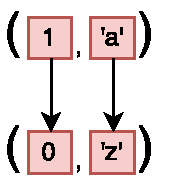
\includegraphics[scale=0.5]{images/parEval2}
\end{center}
\end{frame}
\begin{frame}[fragile] {Map Skeletons (2)}
map, but in \textbf{parallel}:
\begin{lstlisting}[frame=htrbl]
parMap :: conf -> arr a b -> arr [a] [b]
\end{lstlisting}
\begin{center}
\includegraphics[scale=0.5]{images/parMap}
\end{center}
parMap, but \textbf{chunky}:
\begin{lstlisting}[frame=htrbl]
parMapStream :: conf -> ChunkSize -> arr a b -> arr [a] [b]
\end{lstlisting}
\begin{center}
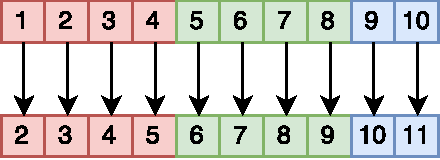
\includegraphics[scale=0.5]{images/parMapStream}
\end{center}
\end{frame}
\begin{frame}[fragile]{Map Skeletons (3)}
parMap, but with \textbf{workload distribution}:
\begin{lstlisting}[frame=htrbl]
farm :: conf -> NumCores -> arr a b -> arr [a] [b]
\end{lstlisting}
\begin{center}
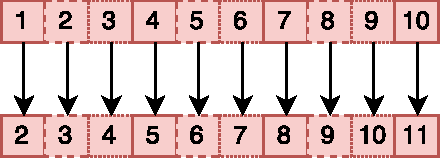
\includegraphics[scale=0.5]{images/farm}
\end{center}
farm, but \textbf{chunky}:
\begin{lstlisting}[frame=htrbl]
farmChunk ::
	conf -> ChunkSize -> NumCores -> arr a b-> arr [a] [b]
\end{lstlisting}
\begin{center}
\includegraphics[scale=0.5]{images/farmChunk}
\end{center}
\end{frame}